%%%%%%%%%%%%%%%%%%%%%%%%%%%%%%%%%%%%%%%%%%%%%%%%%%%%%%%%%%%%%%%%%%%%%%%%%%%%%%%%%%%%%%%%%%%%%%%%
%
% CS484 Written Question Template
%
% Acknowledgements:
% The original code is written by Prof. James Tompkin (james_tompkin@brown.edu).
% The second version is revised by Prof. Min H. Kim (minhkim@kaist.ac.kr).
%
% This is a LaTeX document. LaTeX is a markup language for producing 
% documents. Your task is to fill out this document, then to compile 
% it into a PDF document. 
%
% 
% TO COMPILE:
% > pdflatex thisfile.tex
%
% If you do not have LaTeX and need a LaTeX distribution:
% - Personal laptops (all common OS): www.latex-project.org/get/
% - We recommend latex compiler miktex (https://miktex.org/) for windows,
%   macTex (http://www.tug.org/mactex/) for macOS users.
%   And TeXstudio(http://www.texstudio.org/) for latex editor.
%   You should install both compiler and editor for editing latex.
%   The another option is Overleaf (https://www.overleaf.com/) which is 
%   an online latex editor.
%
% If you need help with LaTeX, please come to office hours. 
% Or, there is plenty of help online:
% https://en.wikibooks.org/wiki/LaTeX
%
% Good luck!
% Min and the CS484 staff
%
%%%%%%%%%%%%%%%%%%%%%%%%%%%%%%%%%%%%%%%%%%%%%%%%%%%%%%%%%%%%%%%%%%%%%%%%%%%%%%%%%%%%%%%%%%%%%%%%
%
% How to include two graphics on the same line:
% 
% \includegraphics[width=0.49\linewidth]{yourgraphic1.png}
% \includegraphics[width=0.49\linewidth]{yourgraphic2.png}
%
% How to include equations:
%
% \begin{equation}
% y = mx+c
% \end{equation}
% 
%%%%%%%%%%%%%%%%%%%%%%%%%%%%%%%%%%%%%%%%%%%%%%%%%%%%%%%%%%%%%%%%%%%%%%%%%%%%%%%%%%%%%%%%%%%%%%%%

\documentclass[11pt]{article}

\usepackage[english]{babel}
\usepackage[utf8]{inputenc}
\usepackage[colorlinks = true,
            linkcolor = blue,
            urlcolor  = blue]{hyperref}
\usepackage[a4paper,margin=1.5in]{geometry}
\usepackage{stackengine,graphicx}
\usepackage{fancyhdr}
\setlength{\headheight}{15pt}
\usepackage{microtype}
\usepackage{times}

% From https://ctan.org/pkg/matlab-prettifier
\usepackage[numbered,framed]{matlab-prettifier}

\frenchspacing
\setlength{\parindent}{0cm} % Default is 15pt.
\setlength{\parskip}{0.3cm plus1mm minus1mm}

\pagestyle{fancy}
\fancyhf{}
\lhead{Homework 3 Questions}
\rhead{CS 484}
\rfoot{\thepage}

\date{}

\title{\vspace{-1cm}Homework 3 Questions}


\begin{document}
\maketitle
\vspace{-3cm}
\thispagestyle{fancy}

\section*{Instructions}
\begin{itemize}
  \item 4 questions.
  \item Write code where appropriate.
  \item Feel free to include images or equations.
  \item Please make this document anonymous.
  \item \textbf{Please use only the space provided and keep the page breaks.} Please do not make new pages, nor remove pages. The document is a template to help grading.
  \item If you really need extra space, please use new pages at the end of the document and refer us to it in your answers.
\end{itemize}

\section*{Questions}

\paragraph{Q1:} Imagine we were tasked with designing a feature point which could match all of the following three pairs of images. Which real world phenomena and camera effects might cause us problems?
Use the MATLAB function \href{https://www.mathworks.com/help/images/ref/corner.html}{$corner$} to investigate. $corner(I,1000)$.

\emph{RISHLibrary} | \emph{Chase} | \emph{LaddObservatory}

%%%%%%%%%%%%%%%%%%%%%%%%%%%%%%%%%%%
\paragraph{A1:} \begin{figure}[!h]
    \centering
    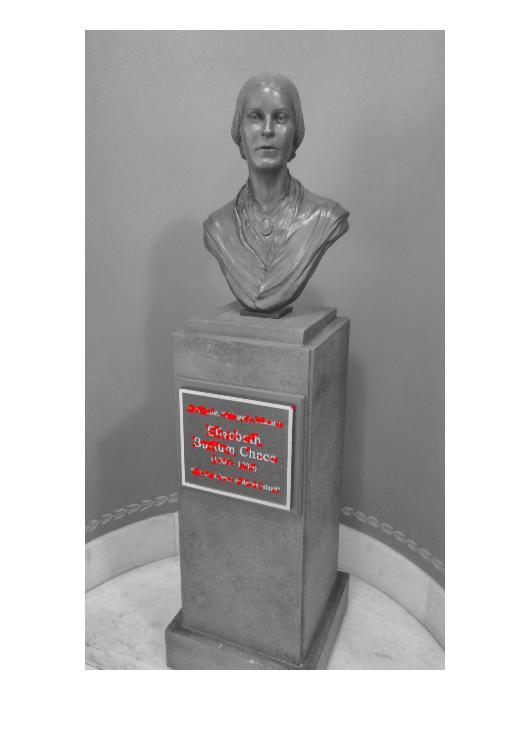
\includegraphics[width=2cm]{q1_Chase1.jpg}
    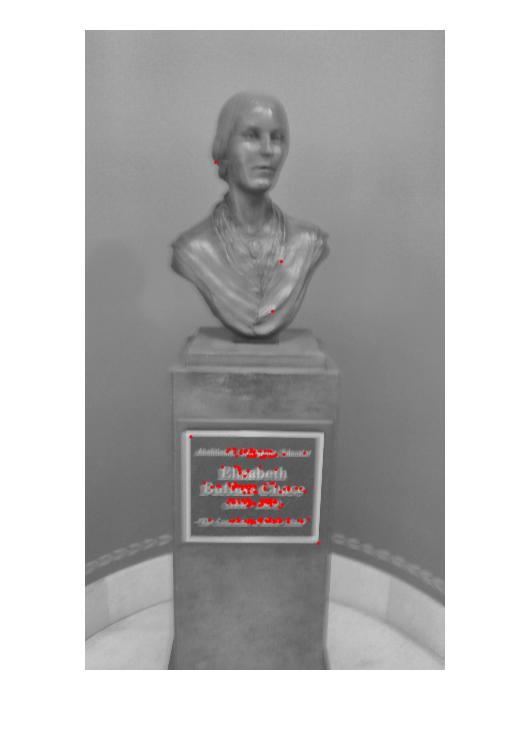
\includegraphics[width=2cm]{q1_Chase2.jpg}
    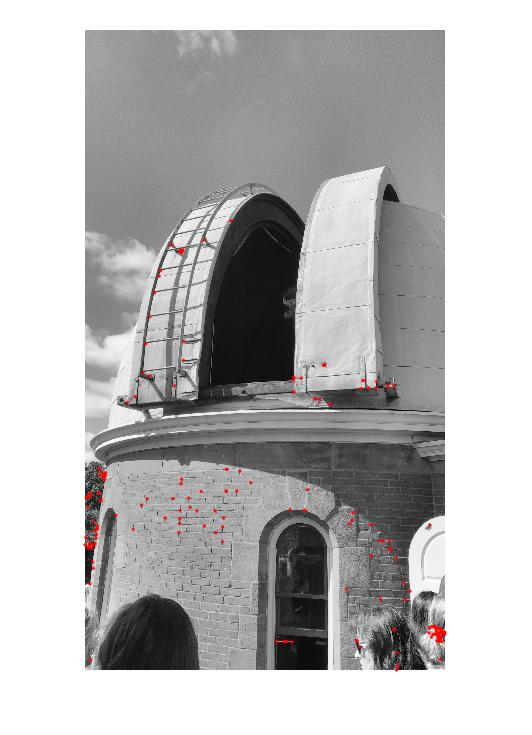
\includegraphics[width=2cm]{q1_LaddObservatory1.jpg}
    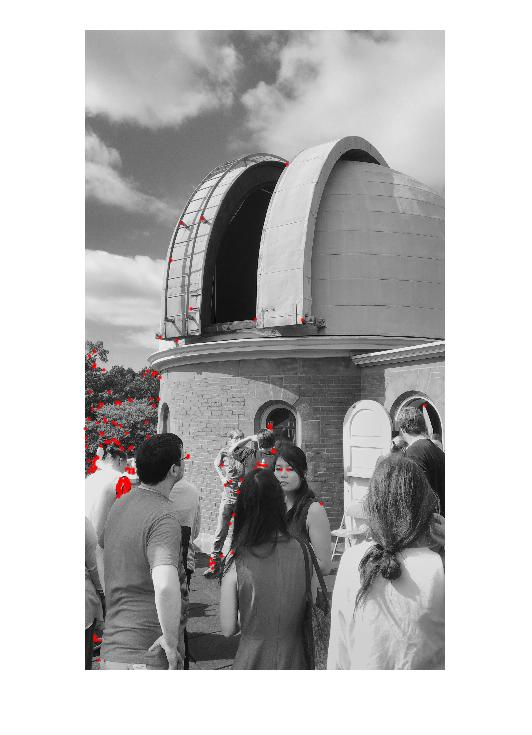
\includegraphics[width=2cm]{q1_LaddObservatory2.jpg}
    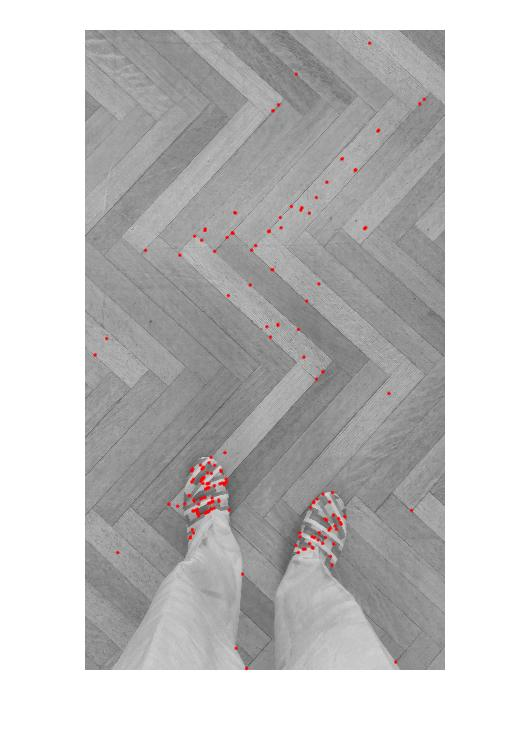
\includegraphics[width=2cm]{q1_RISHLibrary1.jpg}
    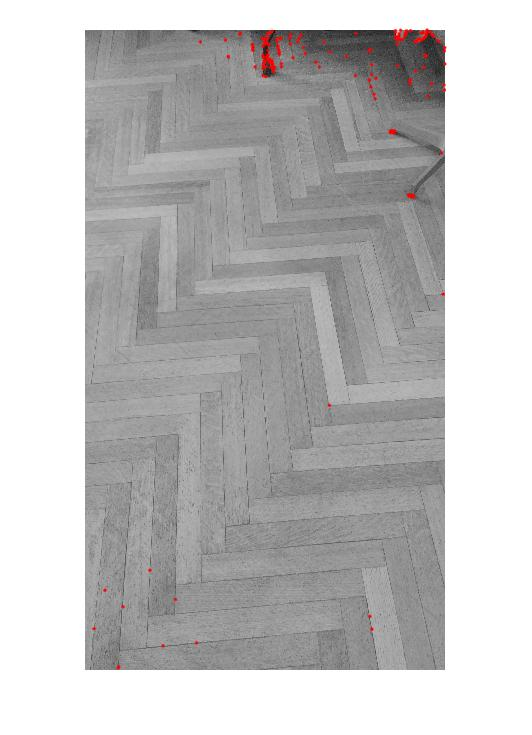
\includegraphics[width=2cm]{q1_RISHLibrary2.jpg}
    \label{fig:pic1}
\end{figure}

In "Chase", photos can be shaken due to a hand shaking situation, and in "LaddObservator" you can see detecting obstacles that are not part of your mind. Finally, in "RISHLibrary," the detailed pattern acts as a noise, so you can see that you cannot detect the desired part with a corner.



%%%%%%%%%%%%%%%%%%%%%%%%%%%%%%%%%%%

% Please leave the pagebreak
\pagebreak
\paragraph{Q2:} In designing our feature point, what characteristics might we wish it to have? Describe the fundamental trade-off between feature point invariance and discriminative power. How should we design for this trade-off?

%%%%%%%%%%%%%%%%%%%%%%%%%%%%%%%%%%%
\paragraph{A2:} If feature point invariance value is high, the discriminative power will be lower, and vice versa, discriminative power is lower. Therefore, if there is a clear demaracation line between the background and the object, give lower the discriminative power. Conversely, if the background is similar to the object, the discriminative power should be high. Like this example, we have to give each image a different value.



%%%%%%%%%%%%%%%%%%%%%%%%%%%%%%%%%%%

% Please leave the pagebreak
\pagebreak
\paragraph{Q3:} In the Harris corner detector, what do the eigenvalues of the 'M' second moment matrix represent? Discuss both how they relate to image intensity and how we can interpret them geometrically.

%%%%%%%%%%%%%%%%%%%%%%%%%%%%%%%%%%%
\paragraph{A3:} This means direction of the slowest change. If there is large diffrence between lambda 1, image is edge. If both of lambda are large, image is corner. And if both of lambda are small, image is flate region.


%%%%%%%%%%%%%%%%%%%%%%%%%%%%%%%%%%%


% Please leave the pagebreak
\pagebreak
\paragraph{Q4:} Explain the difference between the Euclidean distance and the cosine similarity metrics between descriptors. What might their geometric interpretations reveal about when each should be used? Given a distance metric, what is a good method for feature descriptor matching and why?

%%%%%%%%%%%%%%%%%%%%%%%%%%%%%%%%%%%
\paragraph{A4:} If the slimarity cosine matrix meets the condition of positive water space, it is possible to measure distance regardless of dimension.
If you use eucuridean statistics during Feature Matching, you may not be bijective. This problem can be solved to use threshold, but it is difficult to select it. Also, non-distinctive features can be found of close matches, only one of which is correct.



%%%%%%%%%%%%%%%%%%%%%%%%%%%%%%%%%%%


% If you really need extra space, uncomment here and use extra pages after the last question.
% Please refer here in your original answer. Thanks!
%\pagebreak
%\paragraph{AX.X Continued:} Your answer continued here.



\end{document}